% Using IEEEtran class as per Pawsey requirements 
\documentclass[journal]{IEEEtran}

%% PACKAGES %%
\usepackage{newtxtext,newtxmath}
\usepackage{mathrsfs}
\usepackage{graphicx}
\usepackage{subcaption}
\usepackage{multicol}
\usepackage{float}
\usepackage{verbatim}
\usepackage{caption}

\begin{document}

%% DOCUMENT INFO %%
\title{Structural alignment of the nIFTy cluster with cosmic web filaments in the local environment}
\author{Emily Hackett,~\IEEEmembership{Bachelor of Philosophy (Honours) Student, University of Western Australia}}
\markboth{Proceedings of the Pawsey Supercomputing Centre Summer Internships,~Vol.~1, No.~1, February~2017}
{Shell \MakeLowercase{\texit{et al.}}: Alignment of nIFTy cluster with cosmic filaments}

% Make document title
\maketitle

% Report abstract:
\begin{abstract}
	Previous research has shown that the structural properties of dark matter haloes correlate with the local environment of the cosmic web in which they reside (such as filaments, walls and voids). Specifically, by assuming ellipsoid halo shapes, calculation of the inertia tensor for the halo can provide directional information for the major, minor and intermediate axes of the halo. Studies looking at the relationship between these and the halos environment have had varied results for different halo axes and the major filaments, often characterised by some determined misalignment angle. This project makes use of the program DisPerSe to extract the filamentary structure using data from the nIFTy cluster, and by calculating the cluster axes and the filament average direction at the centre of mass of the cluster, determining the misalignment angle as a function of halo radius, for both dark matter and gas components of the cluster (as well as the temperature profile). It was found that no significant alignment was observed between any axes and the calculated filament, likely due to the disrupting effect of a merger within the cluster. The aim of this study was to develop analysis techniques that could hopefully be generalised to much larger data sets, specifically the HorizonAGN simulation, and could also be used to study the alignment of the stellar halo, an area that is increasingly interesting with the advancing capabilities of radio astronomy. 
\end{abstract}

% Introduction:
%	Split into the following subsections
%	1. Background info on cosmological simulations and hierarchical structure formation
%		- What is the cosmic web?
%		- How does large scale structure form?
%	2. Halo structure
%		- What is a cluster/ dark matter halo?
%		- How do we define its structure (briefly talk about angular momentum)
%		- Effects of mergers, tidal effects (showing history of halo - possible
%		  confounding effects for our study

%% DENSITY WITH SKELETON PLOTS %%
\begin{figure*}[t!]
\centering
	\begin{subfigure}[t]{0.3\textwidth}
		\centering
		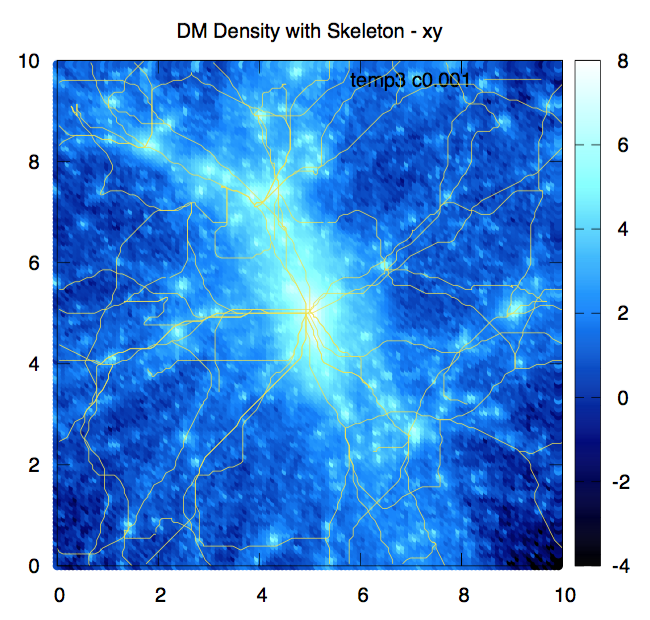
\includegraphics[width=\linewidth]{DMDenSkelxy.png}
	\end{subfigure}
	\quad
	\begin{subfigure}[t]{0.3\textwidth}
		\centering
		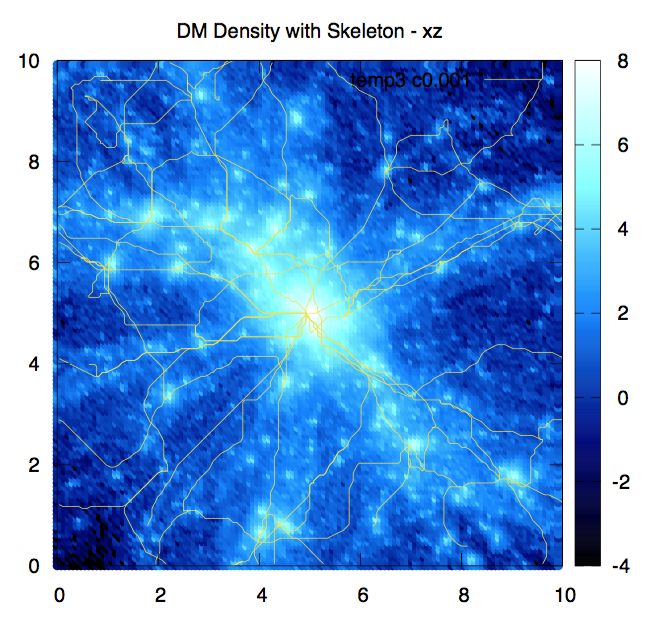
\includegraphics[width=\linewidth]{DMDenSkelxz.png}
	\end{subfigure}
	\quad
	\begin{subfigure}[t]{0.3\textwidth}
		\centering
		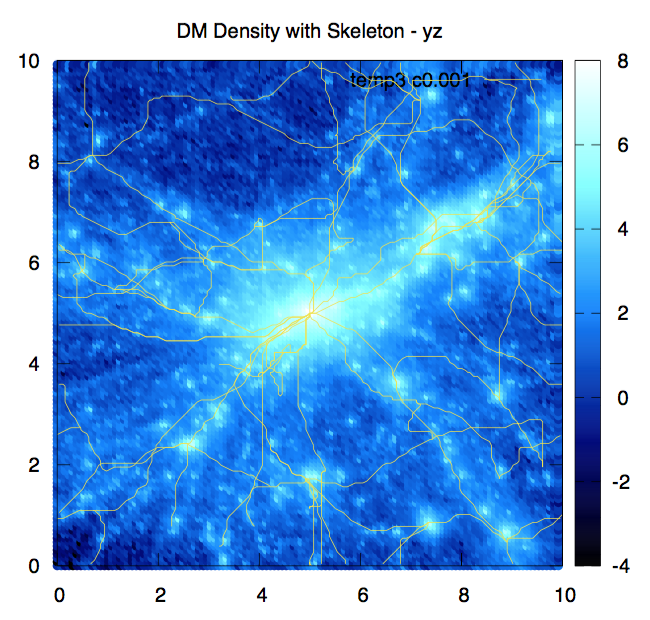
\includegraphics[width=\linewidth]{DMDenSkelyz.png}
	\end{subfigure}
	\\
	\begin{subfigure}[t]{0.3\textwidth}
		\centering
		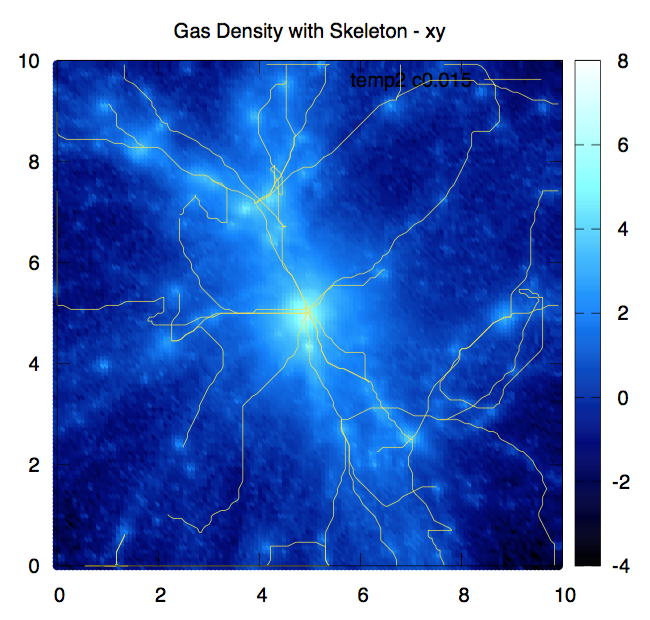
\includegraphics[width=\linewidth]{GasDenSkelxy.png}
	\end{subfigure}
	\quad
	\begin{subfigure}[t]{0.3\textwidth}
		\centering
		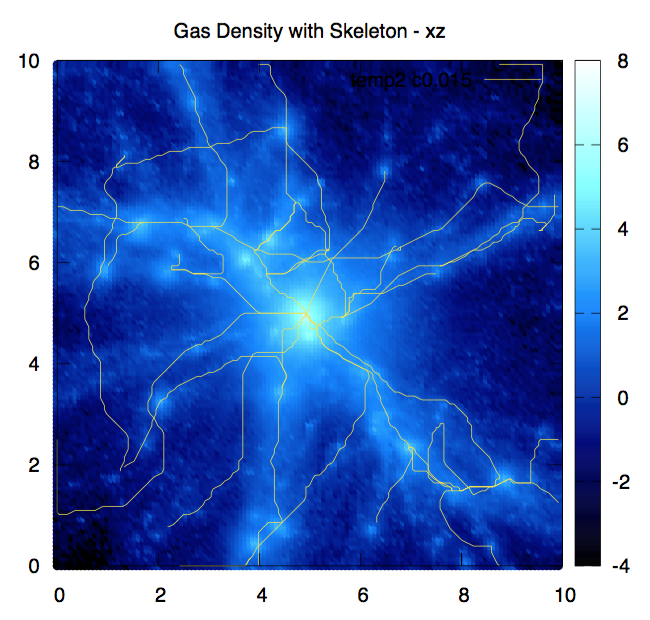
\includegraphics[width=\linewidth]{GasDenSkelxz.png}
	\end{subfigure}
	\quad
	\begin{subfigure}[t]{0.3\textwidth}
		\centering
		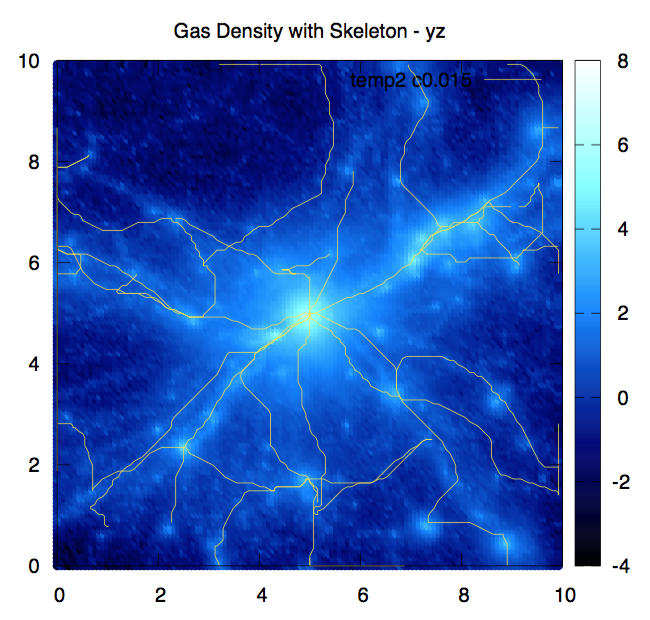
\includegraphics[width=\linewidth]{GasDenSkelyz.png}
	\end{subfigure}
\label{fig:densities}
\caption{Density plots with overlain skeleton for DM and Gas profiles in xy, xz and yz projections.}
\end{figure*}

%% ELLIPSOID PLOTS %%
\begin{figure*}[!t]
\centering
	\begin{subfigure}[t]{0.3\textwidth}
		\centering
		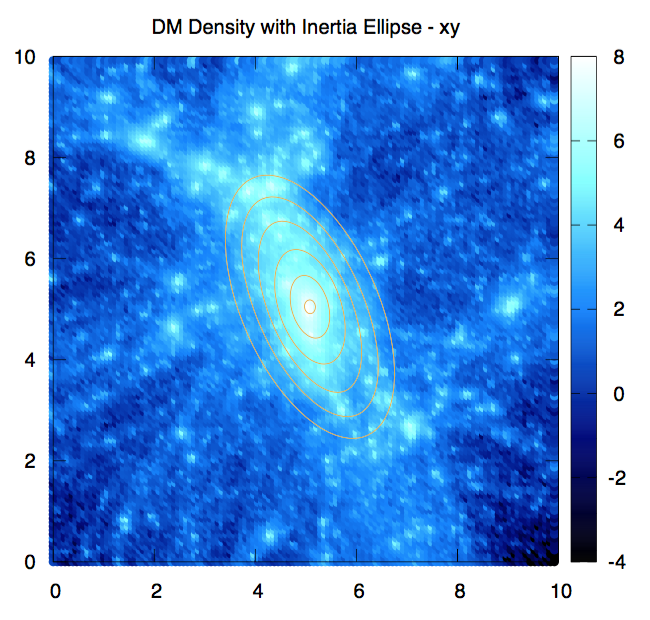
\includegraphics[width=\linewidth]{DMDenEllipxy.png}
	\end{subfigure}
	\quad
	\begin{subfigure}[t]{0.3\textwidth}
		\centering
		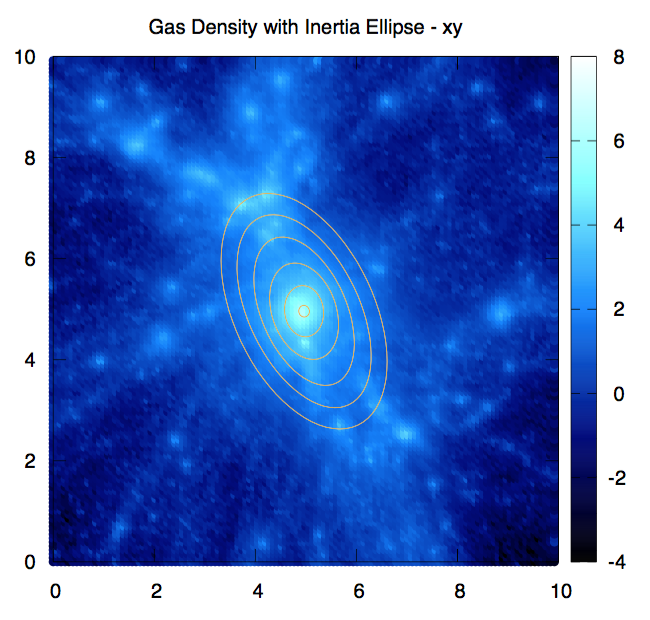
\includegraphics[width=\linewidth]{GasDenEllipxy.png}
	\end{subfigure}
	\quad
	\begin{subfigure}[t]{0.3\textwidth}
		\centering
		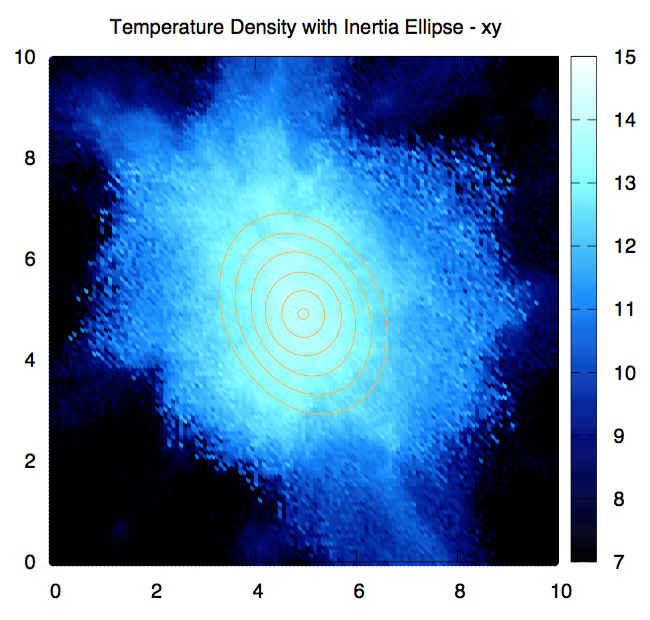
\includegraphics[width=\linewidth]{TempDenEllipxy.png}
	\end{subfigure}
	\\
	\begin{subfigure}[t]{0.3\textwidth}
		\centering
		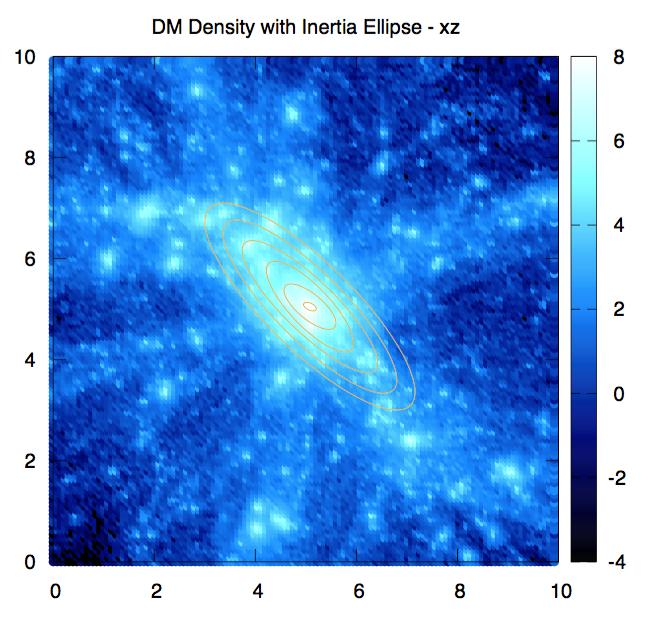
\includegraphics[width=\linewidth]{DMDenEllipxz.png}
	\end{subfigure}
	\quad
	\begin{subfigure}[t]{0.3\textwidth}
		\centering
		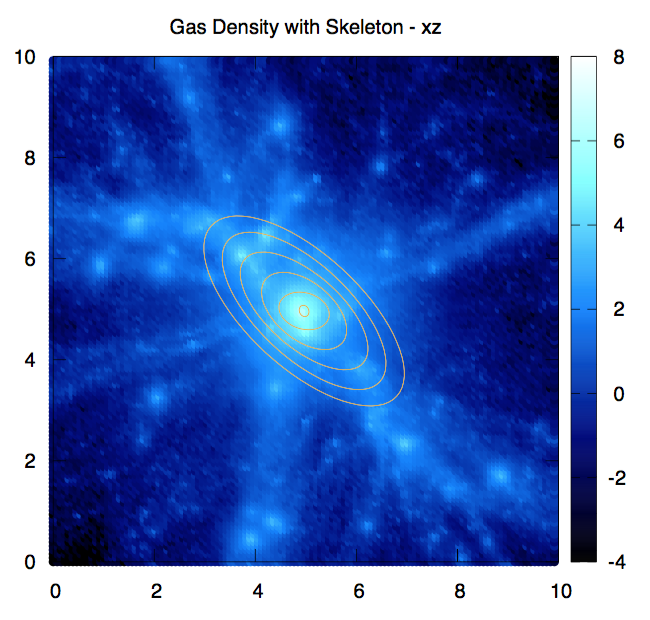
\includegraphics[width=\linewidth]{GasDenEllipxz.png}
	\end{subfigure}
	\quad
	\begin{subfigure}[t]{0.3\textwidth}
		\centering
		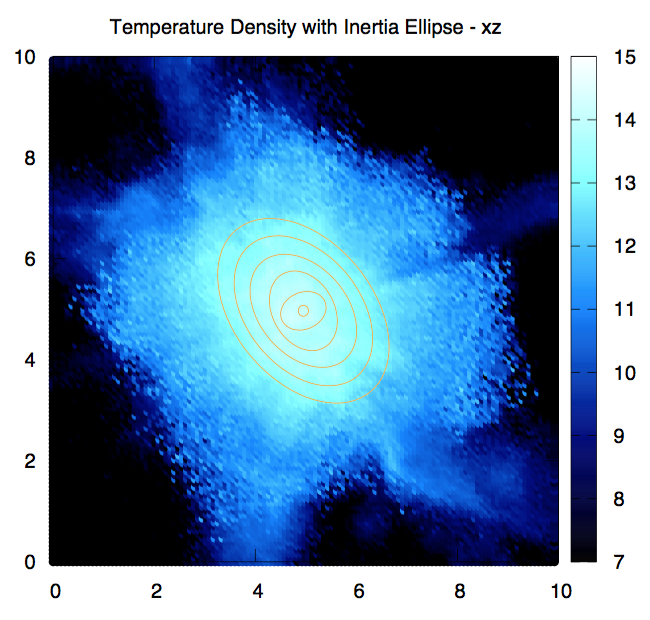
\includegraphics[width=\linewidth]{TempDenEllipxz.png}
	\end{subfigure}
	\\
	\begin{subfigure}[t]{0.3\textwidth}
		\centering
		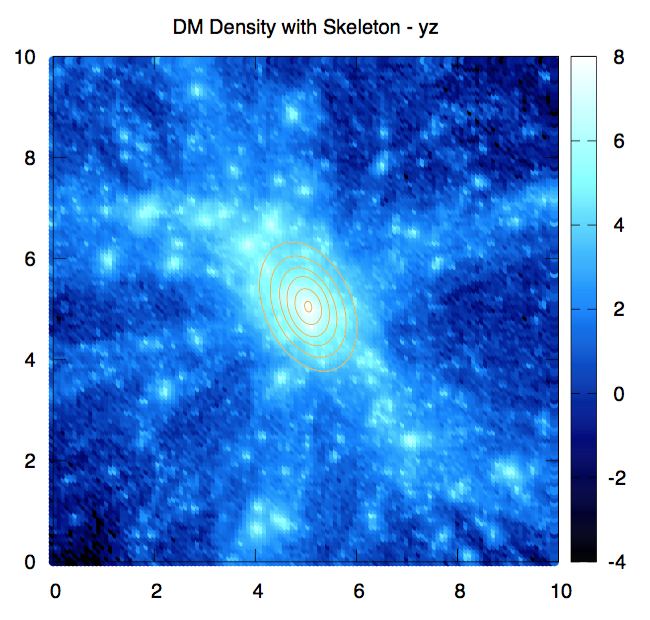
\includegraphics[width=\linewidth]{DMDenEllipyz.png}
	\end{subfigure}
	\quad
	\begin{subfigure}[t]{0.3\textwidth}
		\centering
		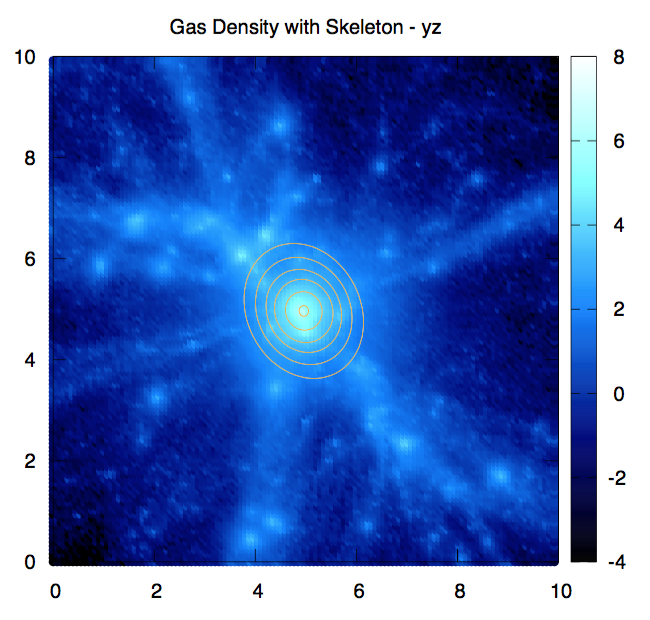
\includegraphics[width=\linewidth]{GasDenEllipyz.png}
	\end{subfigure}
	\quad
	\begin{subfigure}[t]{0.3\textwidth}
		\centering
		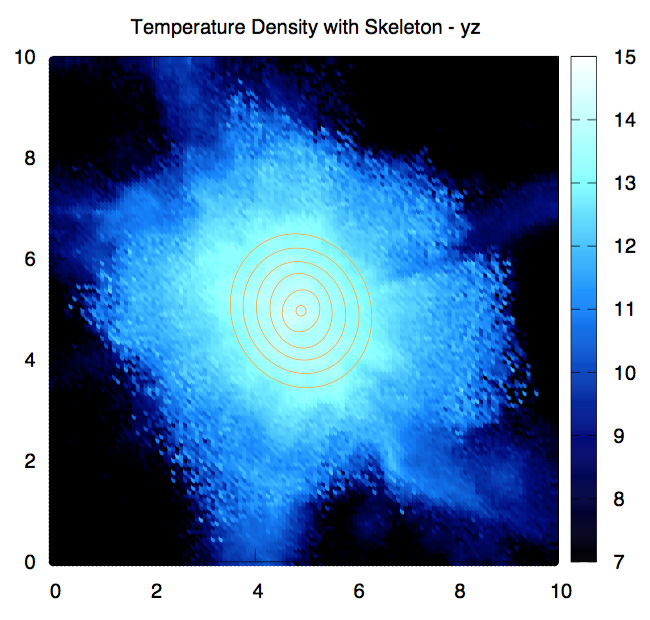
\includegraphics[width=\linewidth]{TempDenEllipyz.png}
	\end{subfigure}
\label{fig:ellipses}
\caption{Ellipses in xy projection for reduced moment of inertia tensor eigenvectors for a) DM, b) gas and c) temperature.}
\end{figure*}

%% SHAPE PLOTS %%
\begin{figure*}[t]
\makebox[\linewidth][c]{
\centering
	\begin{subfigure}[t]{0.37\textwidth}
		\centering
		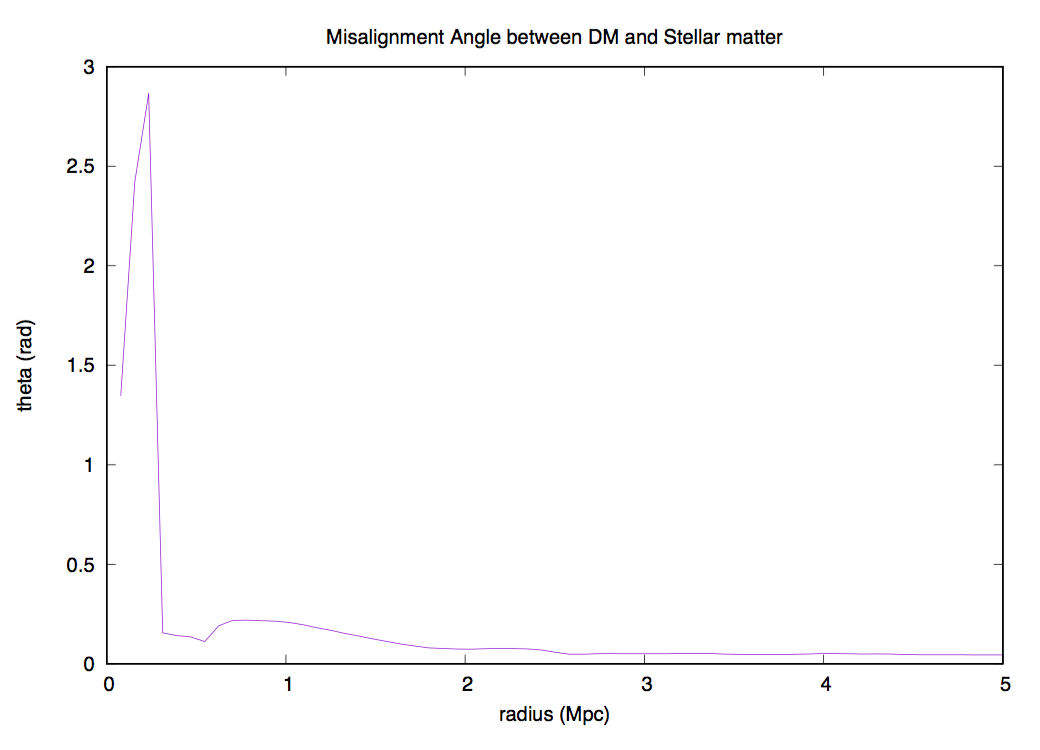
\includegraphics[width=\linewidth]{GasDMAlign.png}
	\end{subfigure}
%	\quad
	\begin{subfigure}[t]{0.37\textwidth}
		\centering
		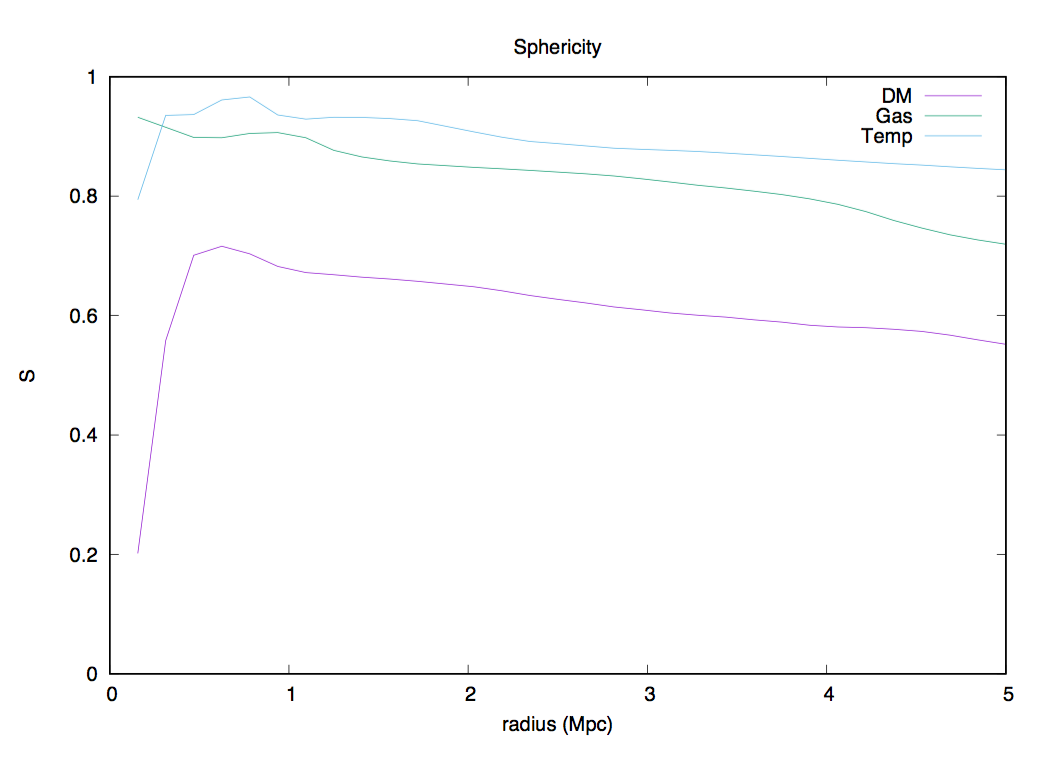
\includegraphics[width=\linewidth]{Sphericity.png}
	\end{subfigure}
%	\quad
%	\begin{subfigure}[t]{0.3\textwidth}
%		\centering
%		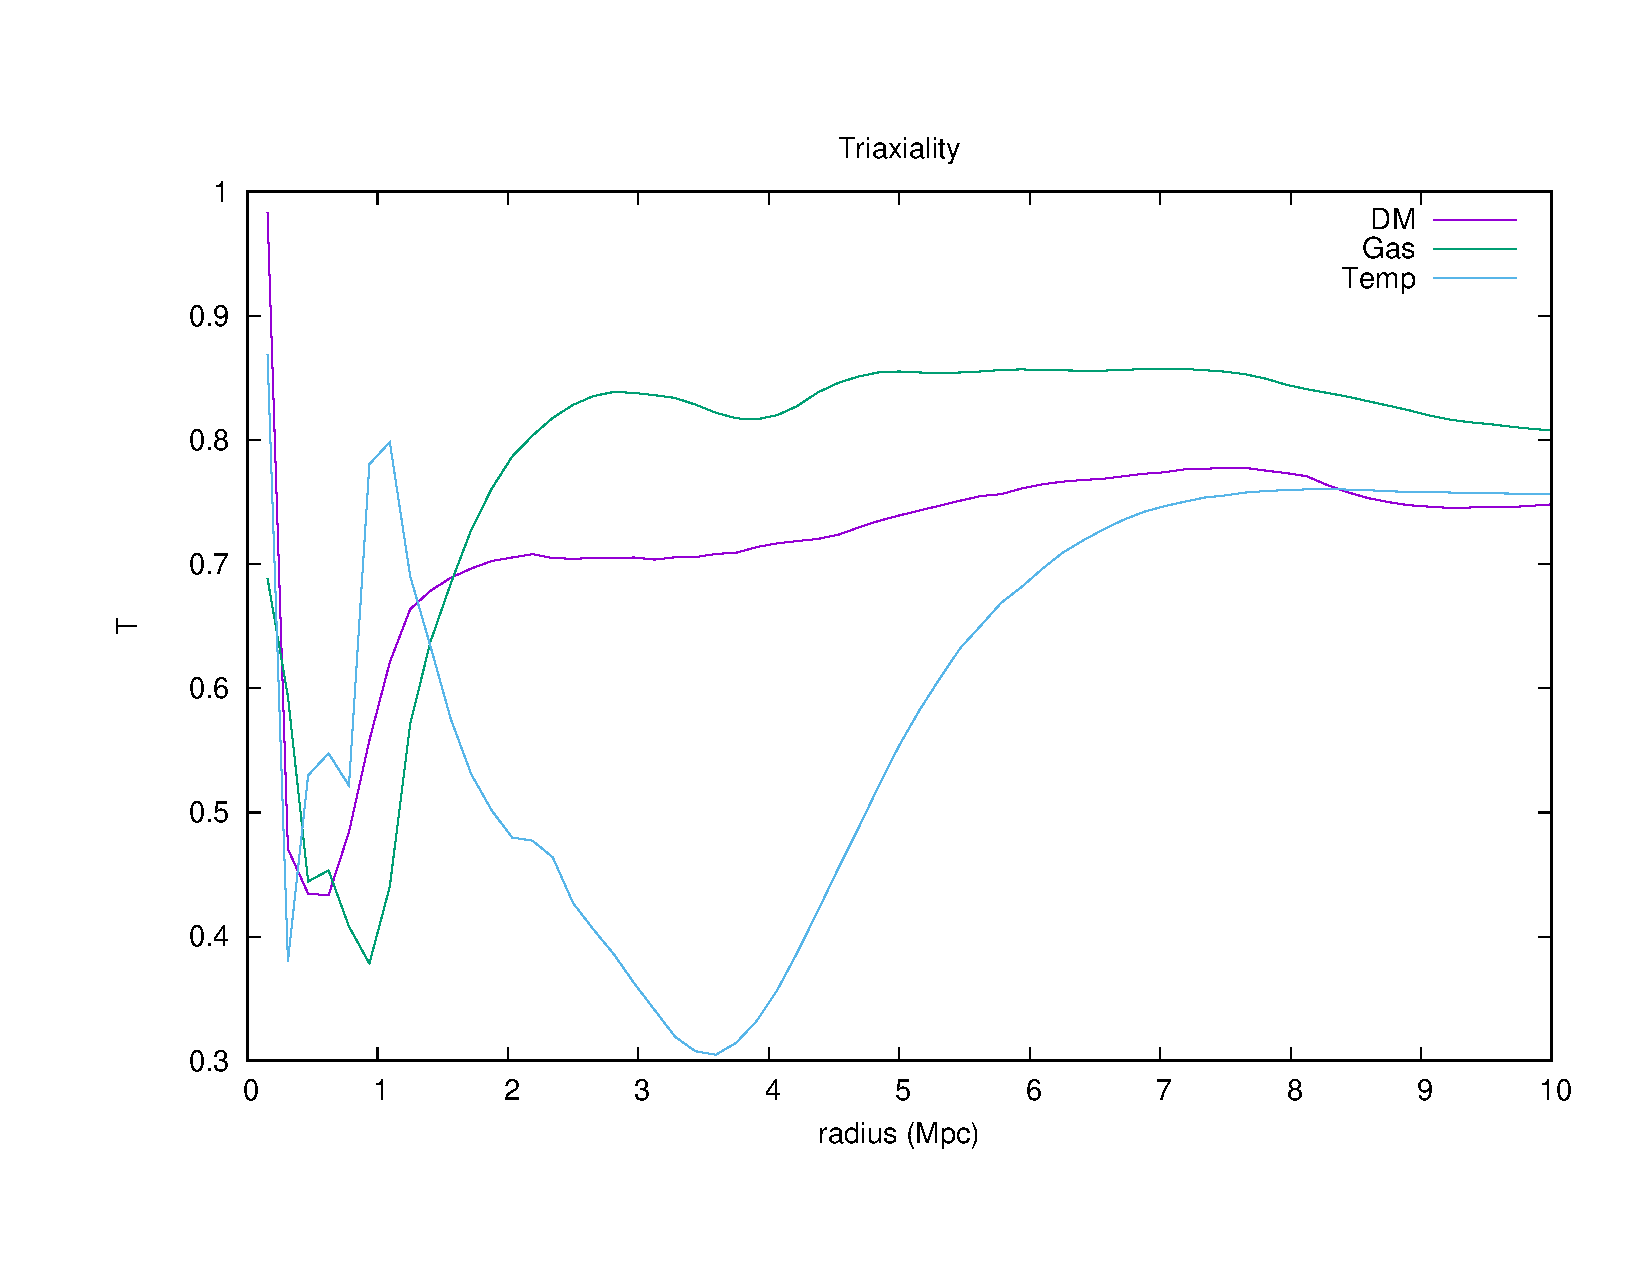
\includegraphics[width=\linewidth]{Triaxiality}
%	\end{subfigure}
%	\quad
	\begin{subfigure}[t]{0.37\textwidth}
		\centering
		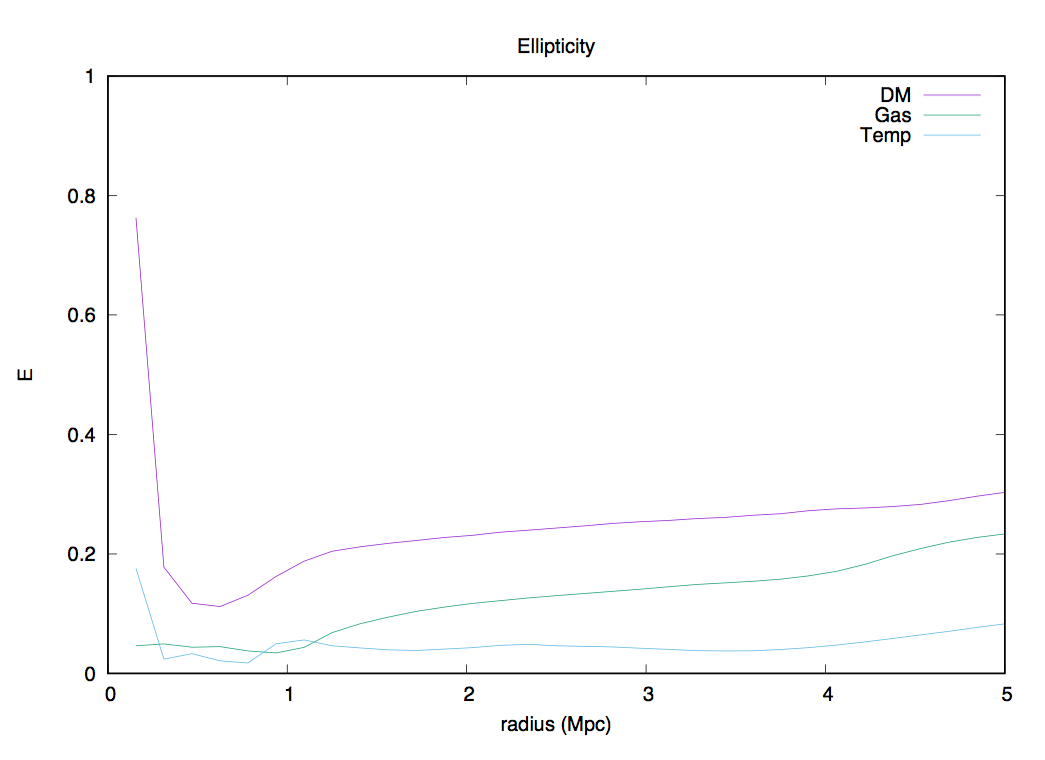
\includegraphics[width=\linewidth]{Ellipticity.png}
	\end{subfigure}
}
\caption{Shape properties of DM, gas and temperature for the halo using a) sphericity and b) ellipticity.}
\label{fig:shapes}
\end{figure*}

\begin{figure*}[t]
\makebox[\linewidth][c]
{
\centering
	\begin{subfigure}[t]{0.55\textwidth}
		\centering
		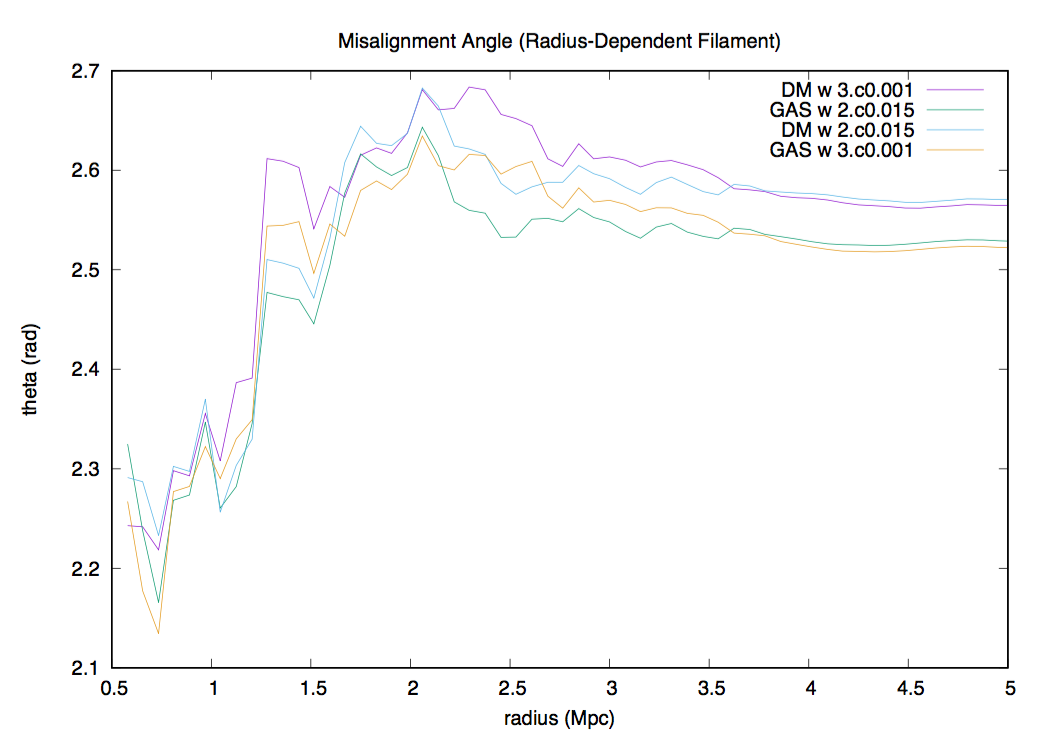
\includegraphics[width=\linewidth]{MisRad.png}
	\end{subfigure}
	\quad
	\begin{subfigure}[t]{0.55\textwidth}
		\centering
		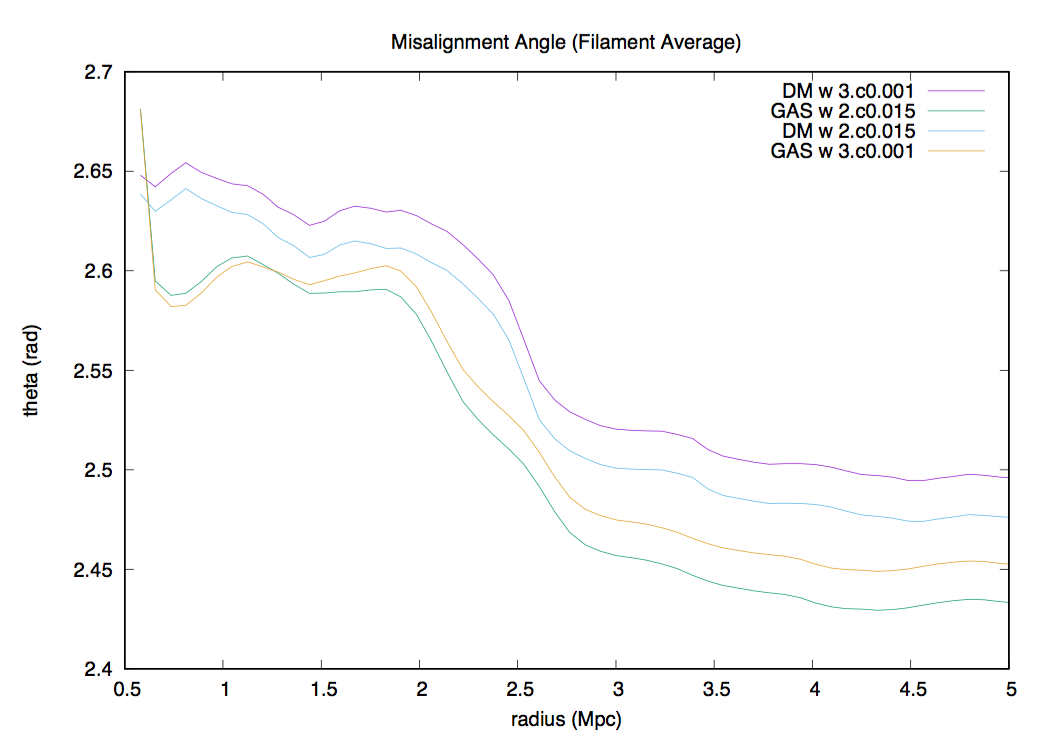
\includegraphics[width=\linewidth]{MisAve.png}
	\end{subfigure}
}
\label{fig:angleplots}
	\caption{Plots of the angle between the filament direction and the major axis for the halo calculated using the reduced moment of inertia tensor at different radii from the centre of mass for a) radius-dependent filament directions and b) the averaged filament direction over all radius.}
\end{figure*}

%% BEGINNING OF PAPER %%
\section{Introduction}
\IEEEPARstart{T}{he} large scale structure of the universe is an area of the utmost importance in investigation of how the universe we see today has come to be. However, since this large scale structure is dominated by dark matter \cite{lemson99} it is not an area easy to image, as galaxies tend to be, so it is commonly investigated through analysis of large cosmological simulations, such as N-body hydrodynamical simulations, assuming a specific 'cosmology' based on how these evolved simulations compare to observations today. The current accepted model for such simulations is the cold dark matter (CDM) cosmology. Simulations in CDM cosmology of the universe demonstrate the growth of large-scale structures, and provide insight on to the hierarchy of structures below them. This map of large-scale structures, which take the form of filaments, sheets and voids, is named the cosmic web.

%\subsection{Hierarchical Structure Formation}
Large scale structure, such as dark matter filaments, clusters and voids, are a general result of nonlinear evolution models in cold dark matter cosmological simulations \cite{davis85}. An example from a recent such study, the Horizon AGN \cite{dubois14}, is pictured in Appendix B, where the filaments are observed as web-like strands, between bright cluster nodes and voids are the empty spaces between them. It is difficult to visualise sheets in the 2D image. Structures build up as a result of merger events, and as these occur, matter is stripped off the merging structures (such as dark matter halos, or on a smaller scale, galaxies) by tidal streams and flows along the larger-scale structure. Therefore since the dark matter halo (and the rest of its matter components) are affected by this structure formation, it makes sense that the halo would exhibit structural correlation with this merger history. Indeed previous research on a variety of simulations show that the halo properties do correlate with its local environment, such as in studies done by Hahn et.al. \cite{hahn07a} \cite{hahn07b}, Lemson and Kauffman \cite{lemson99}and Dubois et.al. with the HorizonAGN simulation \cite{dubois14} among others. 

%\subsection{Halo Properties and Filament Alignment}
 Studies differ in how the local environment is defined, such as Hahn et.al. splitting the environment into clusters, filaments, sheets and voids based on the number of positive eigenvalues of the tidal field tensor, as well as how the halo is characterised. which can be based on either shape or angular momenta. This study will focus on the shape properties of the halos, as calculated using the moment of inertia tensor for the halo, assuming an ellipsoid shape \cite{porciani02a}, using assumptions from tidal torque theory. The eigenvalues of this tensor can be used to calculate the magnitude of the axes of the halo, and its eigenvectors their directions. Specifically, this study focuses on the shape of a single cluster - the nIFTy cluster \cite{nifty}- with the intention of presenting a unified approach to later finding correlations in a large data set, such as the HorizonAGN \cite{dubois14}. The cluster is plotted for dark matter (DM) and gas densities in Figure 1 using 2D slices in the xy, xz and yz planes respectively. 

% Methodology - KEEP FROM PREVIOUS PAPER
\section{Methodology}
\subsection{Reduced Moment of Inertia Tensor}
The physical shape characteristics of the stellar halo can be calculated in a number of different ways, all of which influence the resulting correlations made with the background filament. An important quantity for characterising shape is the moment of inertia tensor, which can be calculated iteratively for a set of particles as per Porciani \cite{porciani02a}. A more useful version is the reduced moment of inertia tensor \cite{tenneti15} which produces a direct correlation between eigenvalues and the principle axes of the assumed elliptic halo. The reduced inertia tensor was calculated for each halo cube according to the following equation:
\begin{equation}
	\tilde{I}_{ij}=\frac{\sum_n m_n \frac{x_{ni}x_{nj}}{r^2_n}}{\sum_n m_n}, \quad \quad \text{where} \quad r^2_n=\sum_i x^2_{ni}
	\label{eq:moitensor}
\end{equation}
Where the generalised $x_i$ coordinates are given with respect to the centre of mass of the halo, which was calculated iteratively for circles of increasingly smaller radii. From this reduced inertia tensor, the eigenvectors represent the principal axes of the halo ellipsoid, and the eigenvalues correspond to the square of the principal axes' lengths. That is, for eigenvalues $\lambda_{a} \geq \lambda_{b} \geq \lambda_{c} $ the lengths of the major, intermediate and minor axes $l_{a},l_{b},l_{c}$ are then $\sqrt{\lambda_{a}}, \sqrt{\lambda_{b}}, \sqrt{\lambda_{c}}$. Note that this only holds because the reduced moment of inertia tensor was calculated.
Since the reduced moment of inertia tensor produces a real symmetric matrix, the eigenvalues and eigenvectors were calculated analytically. 
\subsection{Shape Properties of Stellar Halos}
Using the values for the major, intermediate and minor axes of the elliptic halo, and their corresponding axis vectors, the following quantities were measured. 
\IEEEPARstart{}{Sphericity}: The sphericity of the object is defined with respect to the major and minor axis (the intermediate is ignored). Plotting the sphericity of the stellar and dark matter halo as a function of radius gives an insight into the elongating effects of matter inflow along the filament, and to what extent the halos hold their shape under this force. A spherical halo has sphericity $S=1$ whereas a needle would have $S=0$ \cite{hahn07a}.
\IEEEPARstart{}{Triaxiality}: The triaxiality of the object takes into account all three axes. A prolate halo, one which is lengthened in the direction of its poles, has $T=1$ and an oblate (flattened at the poles) will have $T=0$ \cite{hahn07a}.
\begin{equation}
	S=\frac{l_c}{l_a}, \quad \quad T=\frac{l_a^2-l_b^2}{l_a^2-l_c^2}
	\label{eq:sph&tri}
\end{equation}
\IEEEPARstart{}{Ellipticity}: Perhaps the most significant quantity in regards to this analysis however is the ellipticity, calculated using again only the major and minor axes of the halo. The significance of this comes from the fact the reduced moment of inertia tensor is calculated assuming an ellipsoid body. The ellipticity also gives a measure of how much the halo has been flattened along the filament, ignoring effects of the intermediate axis. The halo would be expected to have more prolate at higher radii as matter streams along the filament to the node.
\begin{equation}
	E=\sqrt{\frac{l_a^2-l_c^2}{l_a^2}}
	\label{eq:ellipticity}
\end{equation}

\subsection{Using DisPerSe to calculate filamentary structure}
The program DisPerSe \cite{sousbie11a}, standing for 'Discrete Persistent Structures Extractor' was developed by Sousbie et.al. to study the properties of filamentary structures in the cosmic web of galaxy distributions, by using the concept of persistence. The main idea is to find persistent topological structures within a data set, which can be of the form of an N-body particle set or a grid with values. These structures are identified as components of Morse-Smale complex of some input function defined over a manifold - this complex captures the relationship between the functions' gradient, its topology, and the topology of the manifold it is defined over. Further detail on this process is given in the Appendix.
The program DisPerSe outputs the skeleton structure for the given data set, which are plotted against the density background in Figure 1. From this skeleton structure, the unit directional vector of the corresponding filament is calculated within differing radii from the centre of mass. Each radii contains all segments from the overall skeleton that have extremities within the given sphere. From here the overall direction of the filament as defined from the centre of mass is calculated by averaging the separate segments. Due to the small number of segments included in any radius smaller than 1 Mpc away from the centre of mass, these filament direction was only calculated for a radius range of 1-5 Mpc. From this set of filament unit vectors, a single averaged filament direction was calculated and used as a constant in further calculations.

\subsection{Pawsey Resources}
The Horizon-AGN data set is located on the Pawsey Supercomputer Magnus in the scratch directory, and is currently being worked on by a PhD student looking to develop a halo-finder algorithm, which would allow these results to be extended to the much larger dataset. The nIFTy cluster is a much smaller dataset, and so this analysis was capable of being conducted on a personal computer. Use was made of the NECTAR research cloud, for computing the reduced moment of inertia tensor and also the centre of mass iteratively. Although no jobs were run on Magnus throughout this project, the skeletons used were originally run on Magnus. 

% Results:
\section{Results}

\subsection{Inertia ellipsoid plots on density background}
As expected, the plots of ellipsoid using the major axes from the eigenvalues of the moment of inertia tensor show significant elongation along the filament direction in all 2D projections, as is expected in the hierarchical model whereby clusters form as matter infalls along the filament. The DM plots show more elliptical shapes than the stellar matter, and the temperature plots maintain a roughly spherical profile throughout, likely corresponding to a virial shock pattern, that could have further effects in the gas and DM profiles. It can be seen that closer to the centre of mass the ellipses become spherical in shape, corresponding to a higher density yet more consistent spread within the smaller radii. 

\subsection{Shape properties for matter and temperature}
The plots of sphericity in Figure \ref{fig:shapes} show that overall the DM in the cube has a lower overall sphericity, with both stellar matter (gas) and temperature profiles showing a higher sphericity. The sphericity for the temperature profile peaks at a radius of approximately 0.8 Mpc out from the halo centre of mass, corresponding to a virial shock seen on the density plots. The stellar matter sphericity peaks slightly further out at a radius of about 1 Mpc, but still related to the temperature peak as would be expected. The higher radius for the Gas profile corresponds to the stellar material being blown out away from the centre of mass by the shock. 
The plot of triaxiality in Figure \ref{fig:shapes} shows significant inconsistency at lower radii, however at higher radii as matter tends to stream along the filament, it is clear that the stellar matter is more elongated along the poles (assumed to be along the filament inflow) whereas the DM is slightly less elongated. The temperature retains a much more spherical profile.
The plot of ellipticity in Figure \ref{fig:shapes} shows that the DM has a higher ellipticty than both stellar matter and the temperature profile. It can be seen that at a radius of about 1 Mpc the temperature briefly has a more elliptic profile than the stellar matter, which corresponds to where the sphericity peaked (which makes sense physically), and can be connected to the virial shock seen on density plots (reference figure that has gas density plotted with circle at centre of mass of radius 1 Mpc). Unlike the temperature profile, the stellar matter increases it's ellipticity until it is almost on par with that of the DM at radius of 5 Mpc (at the edge of the simulation cube), likely due to the fact that 
It is interesting to note the difference between the major axes of the DM and stellar matter, as plotted in Figure \ref{fig:shapes} a). The spike in misalignment at a low radius is likely due to the high sphericity of both matters at very small radii from the centre of mass (as discussed above) which confounds the measurement of an accurate major axis. However there is a noticeable peak at a radius of 1 Mpc out from the centre of mass, the same point at which the temperature profile has higher ellipticity than the gas, i.e. the point at which the gas has an increase in sphericity, corresponding to the blow out of stellar material in a virial shock.

\subsection{Alignment with filament direction}
Overall, the plots of the misalignment angle between major axis and filament in Figure 4 do not show a significant alignment between the two. However the plots still display interesting features. The two methods of filament calculation - that of using an averaged filament, and using an a radius-dependent calculated filament show significant difference at low radius. Due to the smaller number of segments used in calculating at smaller radii (since only those segments completely falling in the given sphere, and not those crossing its boundary, were used) the average filament is assumed to be more accurate here - showing a stronger misalignment at smaller radii). Figure 4 b) also shows a much clearer difference in alignment between dark matter and gas - the gas has a consistently smaller misalignment angle than the dark matter. The slight peak in the gas profile at around 1 Mpc radius matches with similar peaks in the sphericity profile associated with a virial shock. 

% Conclusion:
%	Begin with significance of results (Perhaps put in end of Discussion)
%		- Why is it important to study alignments of halos?
%		  (How we determine more accurate galaxy formation models)
%		- Importance of modelling galaxies (observational studies)
%		  (E.g. weak gravitational lensing)
%		- 

\section{Discussion}
By examining the density plots in Figure 1 and Figure 2, the lack of strong alignment between the major axis of the halo and the filament direction could be attributed to the impact of a significant merger event taking place in the top left corner in the xy 2D slice, as two filaments stream into the main, and there appears to be a cluster of matter at the node of the two. Although clearly visible in the density plot, the effect of such a merger on the differenct shape characteristics plotted in the rest of the paper is unclear. If a study looking at the alignment between halo shape and filamentary structure was to be done on a much larger data set, such as the HorizonAGN (where it would be impossible to study by eye all the density plots of the different halos to try and find major mergers), there would be a need to determine whether such an effect is taking place in any given halo. It would be interesting to see if the misalignment angle was in any way dependent on the number or scale of such events nearby. 
In terms of the analysis undergone here, calculating the reduced inertia tensor, which allows an analytical solution for eigenvalues and eigenvectors, seems to be an accurate and not too computationally expensive method of characterising the halo shape, offering a variety of different insights. More work could be done in characterising the filamentary environment - the calculation of the approximate filament direction could take into use peristence values of the segments, a field value outputted by the DisPerSe program but not used in this analysis. Also segments that were not wholly contained within the bounding radius, but crossing it as well, could be included to provide a larger set within small radii and hopefully more accurate results. 

\section*{Acknowledgment}
I would like to thank both my supervisors, Dr Chris Power and Dr Charlotte Welker, for their assistance on this project and for sharing their valuable time. I would also like to thank Chris Bording, for all his assistance with working with the Pawsey Resources as well as providing such a strong support network for all the studentships. 

%% Appendix
\appendices
\section{The Morse-Smale Complex and Persistence}
Critical points are discrete sets of points where the Morse function's gradient is null, and integral lines are curves tangent to the gradient field at every point. Integral lines cover all space and their extremities are critical points, which induces a tesselation of space into regions called ascending manifolds. The set of these ascending manifolds is the Morse complex of the function. The Morse-Smale complex is an extension of this concept - the space is tesselated into regions called 'p-cells', each of which is the intersection of an ascending and descending manifold. 
Topological components of a function can be represented by pairs of positive and negative critical points called persistence pairs - where a positive critical point corresponds to a created topological component, and a negative to a destroyed topological component. The absolute difference between the value of the critical points in a pair is the persistence, which represents the lifetime of the corresponding component. DisPerSe allows the specification of a persistence threshold which allows removal of topological components with persistence lower, hence filtering noise from the Morse-Smale complex. 

\begin{thebibliography}{1}
\bibitem{lemson99}
	G.~Lemson and G.~Kauffmann, 1999, \emph{Environmental influences on dark matter haloes and consequences for the galaxies within them},\hskip 1em MNRAS 302(1) p.111-117.
\bibitem{davis85}
	M.~Davis,G.~Efstathiou,C.S.~Frenk and S.D.M.~White, 1985, \emph{The evolution of large-scale structure in a universe dominated by cold dark matter}, \hskip 1em The Astrophysical Journal 292 p.371-394.
\bibitem{hahn07a}
	Hahn et.al., 2007, \emph{Properties of dark matter haloes in clusters, filaments, sheets and voids}, \hskip 1em MNRAS 375(2) p.489-499.
\bibitem{hahn07b}
	Hahn et.al., 2007, \emph{The evolution of dark matter halo properties in clusters, filaments, sheets and voids}, \hskip 1em MNRAS 381(1) p.41-51.
\bibitem{dubois14}
	Dubois et.al., 2014, \emph{Dancing in the dark: galactic properties trace spin swings along the cosmic web}, \hskip 1em MNRAS 444(2) p.1453-1468.
\bibitem{porciani02a}
	Porciani et.al., 2002, \emph{Testing tidal-torque theory I. Spin amplitude and direction}, \hskip 1em MNRAS 332(2) p.469-482.
\bibitem{nifty}
	Frederico, S. et.al., 2016, \emph{nIFTy galaxy cluster simulations - II. Radiative models}, \hskip 1em MNRAS 459(3) p.2973-2991.
\bibitem{tenneti15}
	A.~Tenneti, R.~Mandelbaum, T.~Di Matteo, A.~Kiessling and N.~Khandai, 2015, \emph{Galaxy shapes and alignments in the MassiveBlack-II hydrodynamic and dark matter-only simulations}, \hskip 1em MNRAS 453(1) p.469-482.
\bibitem{sousbie11a}
	T.~Sousbie, 2011, \emph{The persistent cosmic web and its filamentary structure - I. Theory and implementation}, \hskip 1em MNRAS 414(1) p.350-383.
\end{thebibliography}

\newpage
\begin{minipage}{2\linewidth}
\section{The Horizon AGN Simulation}
	\centering
	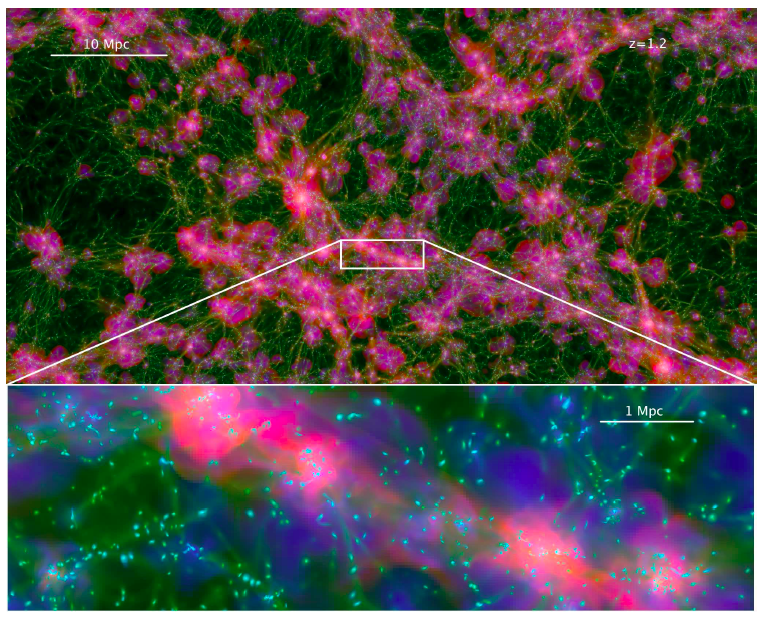
\includegraphics[width=\textwidth]{agnpicture}
	\captionof{figure}{Projected maps of the Horizon AGN simulation, from Dubois et.al. 2014, demonstrating the large-scale structure (filaments, voids and clusters) in the cosmic web. The red demonstrates the temperature shocks in the intergalactic medium around massive halos (of which the nIFTy cluster is also an example of).}
\end{minipage}

\end{document}

